This section describes the data files for a \mf Groundwater Flow (GWF) Model.  A GWF Model is added to the simulation by including a GWF entry in the MODELS block of the simulation name file.

There are three types of spatial discretization approaches that can be used with the GWF Model.  Input for a GWF Model may be entered in a structured form, like for previous MODFLOW versions, in that users specify cells using their layer, row, and column indices.  Users may also work with a layered grid in which cells are defined using vertices.  In this case, users specify cells using the layer number and the cell number.  Lastly, GWF Models may be entered as fully unstructured models, in which cells are specified using only their cell number.  Once a spatial discretization approach has been selected, then all input with cell indices must be entered accordingly.

The GWF Model is designed to permit input to be gathered, as it is needed, from many different files.  Likewise, results from the model calculations can be written to a number of output files. The GWF Model Listing File is a key file to which the GWF model output is written.  As \mf runs, information about the GWF Model is written to the GWF Model Listing File, including much of the input data (as a record of the simulation) and calculated results.  Details about the files used by each package are provided in this section on the GWF Model Instructions.

\mf is further designed to allow the user to control the amount, type, and frequency of information to be output. Much of the output will be written to the Simulation and GWF Model Listing Files, but some model output can be written to other files.  The Listing Files can become very large for common models.  Text editors are useful for examining the Listing File. The GWF Model Listing File includes a summary of the input data read for all packages.  In addition, the GWF Model Listing File optionally contains calculated head controlled by time step, and the overall volumetric budget controlled by time step. The Listing Files also contain information about solver convergence and error messages.  Output to other files can include head and cell-by-cell flow terms for use in calculations external to the model or in user-supplied applications such as plotting programs.

The GWF Model reads a file called the Name File, which specifies most of the files that will be used in a simulation. Several files are always required whereas other files are optional depending on the simulation. The Output Control Package receives instructions from the user to control the amount and frequency of output.  Details about the Name File and the Output Control Package are described in this section.

\subsection{Information for Existing MODFLOW Users}
\mf contains most of the functionality of MODFLOW-2005, MODFLOW-NWT, MODFLOW-USG, and MODFLOW-LGR.  To the existing MODFLOW user, however, \mf will feel different from previous MODFLOW versions.  Some packages have been divided, renamed, or removed, and some capabilities, which previously caused confusion or were implemented due to computer memory limitations, are no longer supported (for example, ``quasi-3d confining units'' are not supported in the GWF Model).  The form of the input files for \mf is different from previous MODFLOW versions in that input files are now divided into blocks, and keywords are used to specify options and input variables.  Extensive testing was used as part of the development process to ensure that \mf simulation results are identical to the results from previous MODFLOW versions.  In some cases, it was not possible to exactly replicate the simulation results from previous MODFLOW versions.  In those cases, the differences could be explained by an option that is no longer supported, or because of slight differences in the underlying formulation.  

The following list has been updated from \cite{modflow6gwf}, and summarizes the major differences between the GWF Model in \mf and previous versions of MODFLOW.  This list is intended for those with a general understanding of the capabilities in previous versions of MODFLOW.

\begin{enumerate}

\item The GWF Model in \mf supports three alternative input packages for specifying the grid used to discretize the groundwater system.  
\begin{itemize}
\item The Discretization (DIS) Package defines a grid based on layers, rows, and columns.  In this report, this type of grid is referred to as a ``regular MODFLOW grid'' because it corresponds to traditional MODFLOW grids.  An interior cell in a regular MODFLOW grid is connected to four adjacent cells in the same layer, to one overlying cell, and to one underlying cell.
\item The Discretization by Vertices (DISV) Package defines a grid using a list of ($x$, $y$) vertex pairs and the number of layers.  A list of vertices is provided by the user to define a two-dimensional horizontal grid in plan view.  This list of vertices may define a regular MODFLOW grid, or they may define more complex grids, such as grids consisting of triangles, hexagons, or Voronoi polygons, for example.  This same two-dimensional horizontal grid applies to each layer in the model.  Cells defined using the DISV Package are referenced by layer number and by the cell number within the horizontal grid.  Within a layer, a cell may be horizontally connected to any number of surrounding cells in that layer.  In the vertical direction a cell can be connected to only one overlying cell and only one underlying cell.  Grids defined with the DISV Package are considered to be unstructured.
\item The unstructured Discretization (DISU) Package is the most flexible of the three packages and is patterned after the unstructured grid implemented in MODFLOW-USG.  For each cell, the user specifies a list of connected cells and the connection properties.  When the DISU Package is used, cells are referenced only by their cell number; unlike the MODFLOW-USG approach, there is no concept of a layer in the DISU Package in \mf, but cells may still overlie or underlie one another.  
\end{itemize}

\item For the three grid types supported in the GWF Model (DIS, DISV, and DISU), cells can be permanently excluded from the grid for the simulation.  Input values (such as hydraulic conductivity) are still required for these excluded cells, and the program will write special codes or zero values for output, but the program does not allocate memory or store values for excluded cells during run time.  In this case, the matrix equations are formulated for a reduced system in which only the included cells are numbered.  Users can also mark excluded cells as ``vertical pass-through cells,'' but this option is only available for DIS and DISV grids.  When these vertical pass-through cells are encountered, the program connects the cells overlying and underlying the pass-through cell.  This capability allows ``pinched'' cells to be removed from the solution.  These options to exclude cells or exclude them as pass-through cells are available through specification of the IDOMAIN array.

\item There is no longer a Basic Package input file.  Initial head values are specified using an Initial Conditions (IC) Package, and constant heads are specified using the Time Varying Specified Head (CHD) Package.  Cells that are permanently excluded from the simulation can be eliminated using the IDOMAIN capability entered through the DIS or DISV Packages.  For a cell that may transition from inactive (``dry'') to active (``wet'') during a simulation, the user can start the cell as inactive by assigning an initial head below the cell bottom.

\item The Newton-Raphson formulations and accompanying upstream weighting schemes implemented in MODFLOW-NWT and MODFLOW-USG for handling dry or nearly dry cells have been synthesized into a single formulation.  The Newton-Raphson formulation in the GWF Model for \mf remains an optional alternative to the standard formulation used in most previous MODFLOW versions. Much of the \cite{modflow6gwf} report is focused on systematically explaining standard and Newton-Raphson formulations for the GWF Model and its packages.

\item Information on temporal discretization, such as number of stress periods, period lengths, number of time steps, and time step multipliers, is specified at the simulation level, rather than for an individual model.  This information is provided in the Timing Module, which controls the temporal discretization and applies to all models within a simulation.  The Timing Module is part of the \mf framework and is described separately in \cite{modflow6framework}.

\item Aquifer properties used to calculate hydraulic conductance are specified in the Node Property Flow (NPF) Package.  In \mf, the NPF Package calculates intercell conductance values, manages cell wetting and drying, and adds Newton-Raphson terms for intercell flow expressions.  The NPF Package allows individual cells to be designated as confined or convertible; this was not an option in previous MODFLOW versions as the designation was by layer.  The NPF Package also has several options for simulating drainage problems and problems involving perched aquifers where an active cell overlies a partially saturated cell.  The default NPF Package behavior (in which none of these options are set) is the most stable for typical groundwater problems.  The default NPF Package behavior does not correspond to the default behavior for other MODFLOW internal flow packages.  The NPF Package does not support quasi-3D confining units.  The NPF Package replaces the Layer Property Flow (LPF), Block-Centered Flow (BCF), and Upstream Weighting (UPW) Packages from previous MODFLOW versions.  Capabilities of the Hydrogeologic Unit Flow (HUF) Package \citep{anderman2000modflow, anderman2003modflow} are not supported in the GWF Model of \mf.

\item Aquifer storage properties are specified in the Storage (STO) Package.  If the STO Package is excluded for a model, then the model represents steady-state conditions.  If the STO Package is included, users can specify steady-state or transient conditions by stress period as needed.  Compressible storage contributions are no longer approximated as zero for unconfined layers; contributions from pore drainage and compressible storage are separated in the model output.

\item The Horizontal Flow Barrier (HFB) Package \citep{hsieh1993hfb, modflow2005} in \mf allows barrier properties and locations to change by stress period.  The capability to change barriers by stress period was not supported in previous MODFLOW versions.

\item The GWF Model in \mf allows multiple stress packages of the same type to be specified for a single GWF Model.  This capability is also available in MODFLOW-CDSS \citep{banta2011modflow}.  Package entries written to the budget file and budget terms in the listing file are written separately for each package.

\item Input of boundary conditions for simulation in multiple stress periods is entered differently than for previous MODFLOW versions. Boundary conditions are specified for a stress period in a ``PERIOD'' block. These boundary conditions remain active at their specified values until a subsequent ``PERIOD'' block is encountered or the end of the simulation is reached.  Individual entries within the ``PERIOD'' block can be specified as a time-series entry.  Values for these variables, which may correspond to a well pumping rate or a drain conductance, for example, are interpolated from a time-series dataset, for each time step, using several different interpolation options.

\item The Flow and Head Boundary (FHB) Package \citep{leake1997documentation, modflow2005} is not supported in \mf; however, its capabilities can be replicated using the WEL Package, the CHD Package, and the new time-series capability.

\item There is one Evapotranspiration (EVT) Package for \mf. The \mf EVT Package contains the functionality of the MODFLOW-2005 EVT Package, the Segmented Evapotranspiration (ETS) Package \citep{modflowdrtpack}, and the Riparian Evapotranspiration (RIP-ET) Package \citep{modflowripetpack}.

\item A new Multi-Aquifer Well (MAW) Package replaces the Multi-Node Well (MNW1 and MNW2) Packages \citep{halford2002, konikow2009}. The new package does not contain all of the options available in MNW1 and MNW2, but it does contain the most commonly used ones.  It also has new capabilities for simulating flowing wells. The MAW Package is solved as part of the matrix solution and is tightly coupled with the GWF Model. This tight coupling with the GWF Model may substantially improve convergence for simulations of groundwater flow to multi-aquifer wells.

\item Most capabilities of the Stream (STR) and Streamflow Routing (SFR) Packages \citep{prudic1989str, modflowsfr1pack, modflowsfr2pack} are included in \mf as a new SFR Package.  The new SFR Package contains all of the functionality of the SFR Package in MODFLOW-2005 with the following exceptions: (a) the concept of a ``segment'' has been eliminated, and (b) unsaturated zone flow beneath stream reaches cannot be simulated.

\item A new Lake (LAK) Package replaces the existing MODFLOW Lake Packages \citep{modflowlak3pack}. In addition to being able to represent lakes that are incised into the model grid, the new LAK Package can also represent sub-grid scale lakes that are conceptualized as being on top of the model.  The status of a lake can change during the simulation between \texttt{ACTIVE}, \texttt{INACTIVE}, and \texttt{CONSTANT}.  The new package contains most of the capabilities available in previous LAK Packages, including the ability to apply recharge and evapotranspiration to underlying cells if the lake is dry.  The LAK Package documented here does not represent unsaturated zone flow beneath a lake or support for the coalescing lake option described in \cite{modflowlak3pack}. 

\item A new Unsaturated Zone Flow (UZF) Package, based on the one described by \cite{UZF}, is included in the GWF Model of \mf. The new UZF Package allows the UZF capabilities to be applied to only selected cells of the GWF model. The new UZF Package also supports a multi-layer option, which allows for vertical heterogeneity in unsaturated zone properties.

\item A new Water Mover (MVR) Package is included in \mf.  The MVR Package can be used to transfer water from individual ``provider'' features of selected packages (WEL, DRN, RIV, GHB, MAW, SFR, LAK, and UZF) to individual ''receiver'' features of the advanced packages (MAW, SFR, LAK, and UZF).  Simple rules are used to determine how much of the available water is moved from the provider to the receiver, which allows management controls to be represented. 

\item A new Skeletal Storage, Compaction, and Subsidence (CSUB) Package was added to \mf in version 6.1.0. The CSUB Package is documented in \cite{modflow6csub}.  The one-dimensional effective-stress based compaction theory implemented in the CSUB Package is based on \cite{leake2007modflow}. The numerical approach used for delay interbeds in the CSUB package is based on \cite{hoffmann2003modflow} and uses the same one-dimensional effective-stress based compaction theory as coarse-grained and fine-grained no-delay interbed sediments.

\item \mf contains a flexible new Observation (OBS) capability, which allows the user to define many different types of continuous-in-time observations.  The new OBS capability replaces the Observation Process \citep{hill2000modflow}, the Gage Package, and the HYDMOD capability \citep{hanson1999documentation} in previous MODFLOW versions.  Flow, head, and drawdown observations can be obtained for the GWF Model.  Flow and other package-specific observations, such as the head in a multi-aquifer well or lake stage, for example, can also be obtained.  These observed values can be used subsequently with a parameter estimation program or they can be used to make time-series plots of a wide range of simulated values.  The new OBS capability does not support specification of field-measured observations, calculation of residuals, or interpolation within a grid, as was supported in previous versions of the MODFLOW OBS Process.

\item The GWF Model described in this report does not support the following list of packages and capabilities.  Support for some of these capabilities may be added in future \mf versions.
  \begin{itemize}
    \item Drain with Return Flow Package \citep{modflowdrtpack},
    \item Reservoir Package \citep{fenske1996documentation},
    \item Seawater Intrusion Package \citep{bakker2013documentation},
    \item Surface-Water Routing Process \citep{hughes2012documentation},
    \item Connected Linear Network Process \citep{modflowusg},
    \item Parameter Value File \citep{modflow2005}, and
    \item Link to the MT3DMS Contaminant Transport Model \citep{zheng2001modflow}.  However, MT3D-USGS can read the head and budget files created by MODFLOW 6, but only if the GWF Model uses the DIS Package.  MT3D-USGS will not work with GWF output if the DISV or DISU Packages are used.
  \end{itemize}

\end{enumerate}

In addition to this list of major differences, there are other differences between \mf and previous MODFLOW versions in terms of the input and output files and the way users interact with the program.  These differences include:

\begin{enumerate}

\item The \mf program begins by reading a simulation name file.  The simulation name file must be named ``mfsim.nam.''

\item All real variables in \mf are declared as double precision floating point numbers.  Real variables written to binary output files are also written in double precision.

\item Unit numbers are no longer specified by the user.  Unit numbers are determined automatically by \mf based upon user-provided file names.

\item The GWF Model name file contains a list of packages that are active for the model.  Names for output files are not specified in the name file.  Names for output files, such as the head and budget files are specified in the OC Package.

\item The EXTERNAL option for reading arrays and lists is no longer supported; however, the OPEN/CLOSE option is still supported.  The SFAC option for lists is no longer supported; however, many packages allow for specification of an auxiliary variable which can serve as a multiplier on a column of values in the list.

\item The CHD Package contains new flexibility.  Cells can transition between constant-head cells and active cells during the simulation.  This was not allowed in previous MODFLOW versions.  Also, the CHD Packages no longer performs linear interpolation between a starting (shead) and ending head (ehead).  Only a single head value is provided for each constant-head cell.  The capability to linearly interpolate a head value for each time step within a stress period is available through the use of time series.

\item There are two different forms of input for the RCH, EVT, SPC, and SPT Packages: array-based input and list-based input.  For models that use DIS Package, input for these packages can be provided as arrays, which is consistent with previous MODFLOW versions.  To use array input, the user must specify the READASARRAYS keyword in the options block.  The READASARRAYS option can also be used for models that use the DISV Package.  If the READASARRAYS option is not specified, then input to the aforementioned packages is provided in list form.  List-based input is the only option supported when the DISU Package is used.

List-based input offers several advantages over the array-based input for specifying recharge and evapotranspiration.  First, multiple list entries can be specified for a single cell.  This makes it possible to divide a cell into multiple areas, and assign a different recharge or evapotranspiration rate for each area (perhaps based on land use or some other criteria).  In this case, the user would likely specify an auxiliary variable to serve as a multiplier.  This multiplier would be calculated by the user and provided in the input file as the fractional cell are for the individual recharge entries.  Another advantage to using list-based input for specifying recharge is that ``boundnames'' can be specified.  Boundnames work with the Observations capability and can be used to sum recharge or evapotranspiration rates for entries with the same boundname.  A disadvantage of the list-based input is that one cannot easily assign recharge or evapotranspiration rates to the entire model without specifying a list of model cells.  For this reason \mf also supports array-based input.

\item Calculation and reporting of drawdown for the model grid is no longer supported, as this calculation is easily performed as a postprocessing step.  Calculation of drawdown is supported as an observation type by the OBS Package; 
drawdown is calculated as the difference between the starting head specified in the IC Package and the calculated head.

\item There are differences in the output files created by \mf, such as:
\begin{itemize}

\item A separate listing file is written for the simulation.  This simulation listing file contains information about the simulation, including solver information.  Separate listing files are written for each GWF Model that is part of the simulation.

\item Unformatted head files written by \mf are consistent with those written by previous MODFLOW versions; however, all real values are written in double precision.

\item The budget file written by the GWF Model is always written in ``compact'' form (as opposed to full three-dimensional arrays) and uses new method codes, which allow model and package names to be written to the file.  Simulated intercell flows are always written in a compressed sparse row format, even for regular MODFLOW grids.

\item Information about the GWF Model grid is written to a separate file, called a ``binary grid file'' each time the model runs.  The binary grid file can be used by postprocessing programs for subsequent analysis.  The format of the binary grid file is described in a section on ``Binary Output Files.''

\end{itemize}


\end{enumerate}


\subsection{Units of Length and Time}
The GWF Model formulates the groundwater flow equation without using prescribed length and time units. Any consistent units of length and time can be used when specifying the input data for a simulation. This capability gives a certain amount of freedom to the user, but care must be exercised to avoid mixing units.  The program cannot detect the use of inconsistent units.  For example, if hydraulic conductivity is entered in units of feet per day and pumpage as cubic meters per second, the program will run, but the results will be meaningless. Other processes generally are expected to work with consistent length and time units; however, other processes could conceivably place restrictions on which units are supported.

The user can set flags that specify the length and time units (see the input instructions for the Timing Module and Spatial Discretization Files), which may be useful in various parts of MODFLOW.  For example, the program will label the table of simulation time with time units if the time units are specified by the optional TIME\_UNITS label, which can be set in the TDIS Package.  If the time units are not specified, the program still runs, but the table of simulation time does not indicate the time units. An optional LENGTH\_UNITS label can be set in the Discretization Package. Situations in other processes may require that the length or time units be specified.  In such situations, the input instructions will state the requirements. Remember that specifying the unit flags does not enforce consistent use of units.  The user must insure that consistent units are used in all input data.

\subsection{Steady-State Simulations}
A steady-state simulation is represented by a single stress period having a single time step with the storage term set to zero. Setting the number and length of stress periods and time steps is the responsibility of the Timing Module of the \mf framework. The length of the stress period and time step will not affect the head solution because the time derivative is not calculated in a steady-state problem. Setting the storage term to zero is the responsibility of the Storage Package. Most other packages need not "know" that a simulation is steady state.

A GWF Model also can be mixed transient and steady state because each stress period can be designated transient or steady state.  Thus, a GWF Model can start with a steady-state stress period and continue with one or more transient stress periods.  The settings for controlling steady-state and transient options are in the Storage Package.  If the Storage Package is not specified for a GWF Model, then the storage terms are zero and the GWF Model will be steady state.

\subsection{Volumetric Budget}
A summary of all inflows (sources) and outflows (sinks) of water is called a water budget.  The water budget for the GWF Model is termed a volumetric budget because volumes of water and volumetric flow rates are involved; thus strictly speaking, a volumetric budget is not a mass balance, although this term has been used in other model reports.  \mf calculates a water budget for the overall model as a check on the acceptability of the solution, and to provide a summary of the sources and sinks of water to the flow system.  The water budget is printed to the GWF Model Listing File for selected time steps.

Numerical solution techniques for simultaneous equations do not always result in a correct answer; in particular, iterative solvers may stop iterating before a sufficiently close approximation to the solution is attained.  A water budget provides an indication of the overall acceptability of the solution.  The system of equations solved by the model actually consists of a flow continuity statement for each model cell.  Continuity should also exist for the total flows into and out of the model---that is, the difference between total inflow and total outflow should equal the total change in storage.  In the model program, the water budget is calculated independently of the equation solution process, and in this sense may provide independent evidence of a valid solution.

The total budget as printed in the output does not include internal flows between model cells---only flows into or out of the model as a whole. For example, flow to or from rivers, flow to or from constant-head cells, and flow to or from wells are all included in the overall budget terms.  Flow into and out of storage is also considered part of the overall budget inasmuch as accumulation in storage effectively removes water from the flow system and storage release effectively adds water to the flow---even though neither process, in itself, involves the transfer of water into or out of the ground-water regime.  Each hydrologic package calculates its own contribution to the budget.

For every time step, the budget subroutine of each hydrologic package calculates the rate of flow into and out of the system due to the process simulated by the package.  The inflows and outflows for each component of flow are stored separately.  Most packages deal with only one such component of flow.  In addition to flow, the volumes of water entering and leaving the model during the time step are calculated as the product of flow rate and time-step length.  Cumulative volumes, from the beginning of the simulation, are then calculated and stored.

The GWF Model uses the inflows, outflows, and cumulative volumes to write the budget to the Listing File at the times requested by the model user.  When a budget is written, the flow rates for the last time step and cumulative volumes from the beginning of simulation are written for each component of flow.  Inflows are written separately from outflows.  Following the convention indicated above, water entering storage is treated as an outflow (that is, as a loss of water from the flow system) while water released from storage is treated as an inflow (that is, a source of water to the flow system).  In addition, total inflow and total outflow are written, as well as the difference between total inflow and outflow.  The difference is then written as a percentage error, calculated using the formula:

\begin{equation}
D = \frac{100 (IN-OUT)}{(IN + OUT) / 2}
\end{equation}

\noindent where $D$ is the percentage error term, $IN$ is the total inflow to the system, and $OUT$ is the total outflow.

If the model equations are solved correctly, the percentage error should be small.  In general, flow rates may be taken as an indication of solution validity for the time step to which they apply, while cumulative volumes are an indication of validity for the entire simulation up to the time of the output.  The budget is written to the GWF Model Listing File at the end of each stress period whether requested or not.

\subsection{Cell-By-Cell Flows}
In some situations, calculating flow terms for various subregions of the model is useful.  To facilitate such calculations, provision has been made to save flow terms for individual cells in a separate binary file so they can be used in computations external to the model itself.  These individual cell flows are referred to here as ``cell-by-cell'' flow terms and are of four general types: (1) cell-by-cell stress flows, or flows into or from an individual cell caused by one of the external stresses represented in the model, such as evapotranspiration or recharge; (2) cell-by-cell storage terms, which give the rate of accumulation or depletion of storage in an individual cell; and (3) internal cell-by-cell flows, which are actually the flows across individual cell faces---that is, between adjacent model cells.  These four kinds of cell-by-cell flow terms are discussed further in subsequent paragraphs.  To save any of these cell-by-cell terms, two flags in the model input must be set.  The input to the Output Control file indicates the time steps for which cell-by-cell terms are to be saved. In addition, each hydrologic package includes an option called SAVE\_FLOWS that must be set if the cell-by-cell terms computed by that package are to be saved.  Thus, if the appropriate option in the Evapotranspiration Package input is set, cell-by-cell evapotranspiration terms will be saved for each time step for which the saving of cell-by-cell flow is requested through the Output Control Option.  Only flow values are saved in the cell-by-cell files; neither water volumes nor cumulative water volumes are included.  The flow dimensions are volume per unit time, where volume and time are in the same units used for all model input data.  The cell-by-cell flow values are stored in unformatted form to make the most efficient use of disk space; see the Budget File section toward the end of this user guide for information on how the data are written to a file.

The cell-by-cell storage term gives the net flow to or from storage in a variable-head cell.  The net storage for each cell in the grid is saved in transient simulations if the appropriate flags are set.  Withdrawal from storage in the cell is considered positive, whereas accumulation in storage is considered negative.

The cell-by-cell constant-head flow term gives the flow into or out of an individual constant-head cell (specified with the CHD Package).  This term is always associated with the constant-head cell itself, rather than with the surrounding cells that contribute or receive the flow.  A constant-head cell may be surrounded by as many as six adjacent variable-head cells for a regular grid or any number of cells for the other grid types.  The cell-by-cell calculation provides a single flow value for each constant-head cell, representing the algebraic sum of the flows between that cell and all of the adjacent variable-head cells.  A positive value indicates that the net flow is away from the constant-head cell (into the variable-head part of the grid); a negative value indicates that the net flow is into the constant-head cell.

The internal cell-by-cell flow values represent flows across the individual faces of a model cell.  Flows between cells are written in the compressed row storage format, whereby the flow between cell $n$ and each one of its connecting $m$ neighbor cells are contained in a single one-dimensional array.  Flows are positive for the cell in question.  Thus the flow reported for cell $n$ and its connection with cell $m$ is opposite in sign to the flow reported for cell $m$ and its connection with cell $n$.  These internal cell-by-cell flow values are useful in calculations of the groundwater flow into various subregions of the model, or in constructing flow vectors.

Cell-by-cell stress flows are flow rates into or out of the model, at a particular cell, owing to one particular external stress.  For example, the cell-by-cell evapotranspiration term for cell $n$ would give the flow out of the model by evapotranspiration from cell $n$.  Cell-by-cell stress flows are considered positive if flow is into the cell, and negative if out of the cell.

\newpage
\subsection{GWF Model Name File}
The GWE Model Name File specifies the options and packages that are active for a GWE model.  The Name File contains two blocks: OPTIONS  and PACKAGES. The length of each line must be 299 characters or less. The lines in each block can be in any order.  Files listed in the PACKAGES block must exist when the program starts. 

Comment lines are indicated when the first character in a line is one of the valid comment characters.  Commented lines can be located anywhere in the file. Any text characters can follow the comment character. Comment lines have no effect on the simulation; their purpose is to allow users to provide documentation about a particular simulation. 

\vspace{5mm}
\subsubsection{Structure of Blocks}
\lstinputlisting[style=blockdefinition]{./mf6ivar/tex/gwe-nam-options.dat}
\lstinputlisting[style=blockdefinition]{./mf6ivar/tex/gwe-nam-packages.dat}

\vspace{5mm}
\subsubsection{Explanation of Variables}
\begin{description}
\input{./mf6ivar/tex/gwe-nam-desc.tex}
\end{description}

\begin{table}[H]
\caption{Ftype values described in this report.  The \texttt{Pname} column indicates whether or not a package name can be provided in the name file.  The capability to provide a package name also indicates that the GWE Model can have more than one package of that Ftype}
\small
\begin{center}
\begin{tabular*}{\columnwidth}{l l l}
\hline
\hline
Ftype & Input File Description & \texttt{Pname}\\
\hline
DIS6 & Rectilinear Discretization Input File \\
DISV6 & Discretization by Vertices Input File \\
DISU6 & Unstructured Discretization Input File \\
FMI6 & Flow Model Interface Package &  \\ 
IC6 & Initial Conditions Package \\
OC6 & Output Control Option \\
ADV6 & Advection Package \\ 
CND6 & Conduction and Dispersion Package \\ 
SSM6 & Source and Sink Mixing Package \\ 
EST6 & Energy Storage and Transfer Package \\
CTP6 & Constant Temperature Package & * \\ 
ESL6 & Energy Source Loading Package & * \\
SFE6 & Streamflow Energy Transport Package & * \\
LKE6 & Lake Energy Transport Package & * \\
MWE6 & Multi-Aquifer Well Energy Transport Package & * \\
UZE6 & Unsaturated-Zone Energy Transport Package & * \\
MVE6 & Mover Energy Transport Package \\
OBS6 & Observations Option \\
\hline 
\end{tabular*}
\label{table:ftype-gwe}
\end{center}
\normalsize
\end{table}

\vspace{5mm}
\subsubsection{Example Input File}
\lstinputlisting[style=inputfile]{./mf6ivar/examples/gwe-nam-example.dat}



\newpage
\subsection{Structured Discretization (DIS) Input File}
\input{gwf/dis}

\newpage
\subsection{Discretization by Vertices (DISV) Input File}
\input{gwf/disv}

\newpage
\subsection{Unstructured Discretization (DISU) Input File}
\input{gwf/disu}

\newpage
\subsection{Initial Conditions (IC) Package}
Initial Conditions (IC) Package information is read from the file that is specified by ``IC6'' as the file type.  Only one IC Package can be specified for a GWF model. 

\vspace{5mm}
\subsubsection{Structure of Blocks}
\lstinputlisting[style=blockdefinition]{./mf6ivar/tex/gwf-ic-options.dat}
\lstinputlisting[style=blockdefinition]{./mf6ivar/tex/gwf-ic-griddata.dat}

\vspace{5mm}
\subsubsection{Explanation of Variables}
\begin{description}
\input{./mf6ivar/tex/gwf-ic-desc.tex}
\end{description}

\vspace{5mm}
\subsubsection{Example Input File}
\lstinputlisting[style=inputfile]{./mf6ivar/examples/gwf-ic-example.dat}



\newpage
\subsection{Output Control (OC) Option}
Input to the Output Control Option of the Groundwater Energy Transport Model is read from the file that is specified as type ``OC6'' in the Name File. If no ``OC6'' file is specified, default output control is used. The Output Control Option determines how and when temperatures are printed to the listing file and/or written to a separate binary output file.  Under the default, temperature and the overall energy transport budget are written to the Listing File at the end of every stress period. The default printout format for temperatures is 10G11.4.  The temperatures and overall energy transport budget are also written to the list file if the simulation terminates prematurely due to failed convergence.

Output Control data must be specified using words.  The numeric codes supported in earlier MODFLOW versions can no longer be used.

For the PRINT and SAVE options of temperature, there is no option to specify individual layers.  Whenever the temperature array is printed or saved, all layers are printed or saved.

\vspace{5mm}
\subsubsection{Structure of Blocks}
\vspace{5mm}

\noindent \textit{FOR EACH SIMULATION}
\lstinputlisting[style=blockdefinition]{./mf6ivar/tex/gwe-oc-options.dat}
\vspace{5mm}
\noindent \textit{FOR ANY STRESS PERIOD}
\lstinputlisting[style=blockdefinition]{./mf6ivar/tex/gwe-oc-period.dat}

\vspace{5mm}
\subsubsection{Explanation of Variables}
\begin{description}
\input{./mf6ivar/tex/gwe-oc-desc.tex}
\end{description}

\vspace{5mm}
\subsubsection{Example Input File}
\lstinputlisting[style=inputfile]{./mf6ivar/examples/gwe-oc-example.dat}


\newpage
\subsection{Observation (OBS) Utility for a GWF Model}
\input{gwf/gwf-obs}

\newpage
\subsection{Node Property Flow (NPF) Package}
\input{gwf/npf}

\newpage
\subsection{Time-Varying Hydraulic Conductivity (TVK) Package}
\input{gwf/tvk}

\newpage
\subsection{Horizontal Flow Barrier (HFB) Package}
\input{gwf/hfb}

\newpage
\subsection{Storage (STO) Package}
Input to the Storage (STO) Package is read from the file that has type ``STO6'' in the Name File.  If the STO Package is not included for a model, then storage changes will not be calculated, and thus, the model will be steady state.  Only one STO Package can be specified for a OLF model.

\vspace{5mm}
\subsubsection{Structure of Blocks}

\vspace{5mm}
\noindent \textit{FOR EACH SIMULATION}
\lstinputlisting[style=blockdefinition]{./mf6ivar/tex/olf-sto-options.dat}
\vspace{5mm}
\noindent \textit{FOR ANY STRESS PERIOD}
\lstinputlisting[style=blockdefinition]{./mf6ivar/tex/olf-sto-period.dat}

\vspace{5mm}
\subsubsection{Explanation of Variables}
\begin{description}
\input{./mf6ivar/tex/olf-sto-desc.tex}
\end{description}

\vspace{5mm}
\subsubsection{Example Input File}
\lstinputlisting[style=inputfile]{./mf6ivar/examples/olf-sto-example.dat}



\newpage
\subsection{Time-Varying Storage (TVS) Package}
\input{gwf/tvs}

\newpage
\subsection{Skeletal Storage, Compaction, and Subsidence (CSUB) Package}
Input to the Skeletal Storage, Compaction, and Subsidence (CSUB) Package is read from the file that has type ``CSUB6'' in the Name File.  Technical details for the CSUB Package are described in \cite{modflow6csub}.  If the CSUB Package is not included for a model, then storage changes resulting from compaction will not be calculated.  Only one CSUB Package can be specified for a GWF model. Only the first and last stress period can be specified to be STEADY-STATE in the STO Package when the CSUB Package is being used in the GWF model. Also the specific storage (SS) must be specified to be zero in the STO Package for every cell.

\vspace{5mm}
\subsubsection{Structure of Blocks}

\vspace{5mm}
\noindent \textit{FOR EACH SIMULATION}
\lstinputlisting[style=blockdefinition]{./mf6ivar/tex/gwf-csub-options.dat}
\lstinputlisting[style=blockdefinition]{./mf6ivar/tex/gwf-csub-dimensions.dat}
\lstinputlisting[style=blockdefinition]{./mf6ivar/tex/gwf-csub-griddata.dat}
\lstinputlisting[style=blockdefinition]{./mf6ivar/tex/gwf-csub-packagedata.dat}
\vspace{5mm}
\noindent \textit{FOR ANY STRESS PERIOD}
\lstinputlisting[style=blockdefinition]{./mf6ivar/tex/gwf-csub-period.dat}
\packageperioddescription

\vspace{5mm}
\subsubsection{Explanation of Variables}
\begin{description}
\input{./mf6ivar/tex/gwf-csub-desc.tex}
\end{description}

\vspace{5mm}
\subsubsection{Example Input File}
\lstinputlisting[style=inputfile]{./mf6ivar/examples/gwf-csub-example.dat}


\vspace{5mm}
\subsubsection{Available observation types}
Subsidence Package observations include all of the terms that contribute to the continuity equation for each GWF cell. The data required for each CSUB Package observation type is defined in table~\ref{table:gwf-csubobstype}. Negative and positive values for \texttt{CSUB} observations represent a loss from and gain to the GWF model, respectively.


\begin{longtable}{p{2cm} p{2.75cm} p{2cm} p{1.25cm} p{7cm}}
\caption{Available CSUB Package observation types} \tabularnewline

\hline
\hline
\textbf{Stress Package} & \textbf{Observation type} & \textbf{ID} & \textbf{ID2} & \textbf{Description} \\
\hline
\endfirsthead

\captionsetup{textformat=simple}
\caption*{\textbf{Table \arabic{table}.}{\quad}Available CSUB Package observation types.---Continued} \\

\hline
\hline
\textbf{Stress Package} & \textbf{Observation type} & \textbf{ID} & \textbf{ID2} & \textbf{Description} \\
\hline
\endhead

\hline
\multicolumn{5}{l}{\textbf{NOTE}: The NODATA value is reported for steady-state stress periods.} \\
\endfoot

CSUB & csub & icsubno or boundname & -- & Flow between the groundwater system and a interbed or group of interbeds. \\
CSUB & inelastic-csub & icsubno or boundname & -- & Flow between the groundwater system and a interbed or group of interbeds from inelastic compaction. \\
CSUB & elastic-csub & icsubno or boundname & -- & Flow between the groundwater system and a interbed or group of interbeds from elastic compaction. \\
CSUB & coarse-csub & cellid & -- & Flow between the groundwater system and coarse-grained materials in a GWF cell. \\
CSUB & csub-cell & cellid & -- & Flow between the groundwater system for all interbeds and coarse-grained materials in a GWF cell. \\
CSUB & wcomp-csub-cell & cellid & -- & Flow between the groundwater system for all interbeds and coarse-grained materials in a GWF cell from water compressibility. \\

CSUB & sk & icsubno & -- & Convertible interbed storativity in a interbed. Convertible interbed storativity is inelastic interbed storativity if the current effective stress is greater than the preconsolidation stress. \\
CSUB & ske & icsubno & -- & Elastic interbed storativity in a interbed. \\
CSUB & sk-cell & cellid & -- & Convertible interbed and coarse-grained material storativity in a GWF cell. Convertible interbed storativity is inelastic interbed storativity if the current effective stress is greater than the preconsolidation stress. \\
CSUB & ske-cell & cellid & -- & Elastic interbed and coarse-grained material storativity in a GWF cell. \\

CSUB & estress-cell & cellid & -- & effective stress in a GWF cell. \\
CSUB & gstress-cell & cellid & -- & geostatic stress in a GWF cell. \\

CSUB & interbed-compaction & icsubno  & -- & interbed compaction in a interbed. \\
CSUB & inelastic-compaction &  icsubno & -- & inelastic interbed compaction in a interbed. \\
CSUB & elastic-compaction &  icsubno & -- & elastic interbed compaction a interbed. \\
CSUB & coarse-compaction & cellid  & -- & elastic compaction in coarse-grained materials in a GWF cell. \\
CSUB & inelastic-compaction-cell &  cellid & -- & inelastic compaction in all interbeds in a GWF cell. \\
CSUB & elastic-compaction-cell &  cellid & -- & elastic compaction in coarse-grained materials and all interbeds in a GWF cell. \\
CSUB & compaction-cell & cellid  & -- & total compaction in coarse-grained materials and all interbeds in a GWF cell. \\

CSUB & thickness & icsubno & -- & thickness of a interbed. \\
CSUB & coarse-thickness & cellid & -- & thickness of coarse-grained materials in a GWF cell. \\
CSUB & thickness-cell & cellid & -- & total thickness of coarse-grained materials and all interbeds in a GWF cell. \\

CSUB & theta & icsubno & -- & porosity of a interbed. \\
CSUB & coarse-theta & cellid  & -- & porosity of coarse-grained materials in a GWF cell. \\
CSUB & theta-cell & cellid  & -- & thickness-weighted porosity of coarse-grained materials and all interbeds in a GWF cell. \\

CSUB & delay-flowtop & icsubno or boundname  & -- & Flow between the groundwater system and a delay interbed or group of interbeds across the top of the interbed(s). \\
CSUB & delay-flowbot & icsubno or boundname  & -- & Flow between the groundwater system and a delay interbed or group of interbeds across the bottom of the interbed(s). \\

CSUB & delay-head & icsubno & idcellno & head in interbed in delay cell idcellno (1 $<=$ idcellno $<=$ NDELAYCELLS). \\
CSUB & delay-gstress & icsubno  & idcellno & geostatic stress in interbed in delay cell idcellno (1 $<=$ idcellno $<=$ NDELAYCELLS). \\
CSUB & delay-estress & icsubno  & idcellno & effective stress in interbed in delay cell idcellno (1 $<=$ idcellno $<=$ NDELAYCELLS). \\
CSUB & delay-preconstress & icsubno  & idcellno & preconsolidation stress in interbed in delay cell idcellno (1 $<=$ idcellno $<=$ NDELAYCELLS). \\
CSUB & delay-compaction & icsubno  & idcellno & compaction in interbed in delay cell idcellno (1 $<=$ idcellno $<=$ NDELAYCELLS). \\
CSUB & delay-thickness & icsubno  & idcellno & thickness of interbed or group of interbeds in delay cell idcellno (1 $<=$ idcellno $<=$ NDELAYCELLS). \\
CSUB & delay-theta & icsubno  & idcellno & porosity of interbed in delay cell idcellno (1 $<=$ idcellno $<=$ NDELAYCELLS). \\

CSUB & preconstress-cell & cellid  & -- & preconsolidation stress in a GWF cell containing at least one interbed.

\label{table:gwf-csubobstype}
\end{longtable}

\vspace{5mm}
\subsubsection{Example Observation Input File}
\lstinputlisting[style=inputfile]{./mf6ivar/examples/gwf-csub-example-obs.dat}

\newpage
\subsection{Buoyancy (BUY) Package}
\input{gwf/buy}

\newpage
\subsection{Viscosity (VSC) Package}
Input to the Viscosity (VSC) Package is read from the file that has type ``VSC6'' in the Name File.  If the VSC Package is active within a groundwater flow model, then the model will account for the dependence of fluid viscosity on solute concentration and the resulting changes in hydraulic conductivity and stress-package conductances, which vary inversely with viscosity.  Viscosity can be calculated as a function of one or more groundwater solute transport (GWT) species using an approach described in the Supplemental Technical Information document distributed with MODFLOW 6 (Chapter 8).  Only one VSC Package can be specified for a GWF model. The VSC Package can be coupled with one or more GWT Models so that the fluid viscosity is updated dynamically with one or more simulated concentration fields.

The VSC Package calculates fluid viscosity using the following equation from \cite{langevin2008seawat}:

\begin{equation}
\label{eqn:visclinear}
\mu = VISCREF + \sum_{i=1}^{NVISCSPECIES} DVISCDC_i \left ( CONCENTRATION_i - CVISCREF_i \right )
\end{equation}

\noindent where $\mu$ is the calculated viscosity, $VISCREF$ is the viscosity of a reference fluid, typically taken to be freshwater at a temperature of 20 degrees Celsius, $NVISCSPECIES$ is the number of chemical species that contribute to the viscosity calculation, $DVISCDC_i$ is the parameter that describes how viscosity changes linearly as a function of concentration for chemical species $i$ (i.e. the slope of a line that relates viscosity to concentration), $CONCENTRATION_i$ is the concentration of species $i$, and $CVISCREF_i$ is the reference concentration for species $i$ corresponding to when the viscosity of the reference fluid is equal to $VISCREF$, which is normally set to a concentration of zero.

In many applications, variations in temperature have a greater effect on fluid viscosity than variations in solute concentration. When a GWT model is formulated such that one of the transported ``species'' is heat (thermal energy), with ``concentration'' used to represent temperature \citep{zheng2010supplemental}, the viscosity can vary linearly with temperature, as it can with any other ``concentration.''  In that case, $CONCENTRATION_i$ and $CVISCREF_i$ represent the simulated and reference temperatures, respectively, and $DVISCDC_i$ represents the rate at which viscosity changes with temperature. In addition, the viscosity formula can optionally include a nonlinear dependence on temperature. In that case, equation 3 becomes

\begin{equation}
\label{eqn:viscnonlinear}
\mu = \mu_T(T) + \sum_{i=1}^{NVISCSPECIES} DVISCDC_i \left ( CONCENTRATION_i - CVISCREF_i \right )
\end{equation}

\noindent where the first term on the right-hand side, $\mu_T(T)$, is a nonlinear function of temperature, and the summation corresponds to the summation in equation \ref{eqn:visclinear}, in which one of the ``species'' is heat. The nonlinear term in equation \ref{eqn:viscnonlinear} is of the form

\begin{equation}
\label{eqn:munonlinear}
\mu_T(T) = CVISCREF_i \cdot A_2^{\left [ \frac {-A_3 \left ( CONCENTRATION_i - CVISCREF_i \right ) } {\left ( CONCENTRATION_i + A_4 \right ) \left ( CVISCREF_i + A_4 \right )} \right ]}
\end{equation}

\noindent where the coefficients $A_2$, $A_3$, and $A_4$ are specified by the user.  Values for $A_2$, $A_3$, and $A_4$ are commonly 10, 248.7, and 133.15, respectively  \citep{langevin2008seawat, Voss1984sutra}.
 
\subsubsection{Stress Packages}

For head-dependent stress packages, the VSC Package can adjust the conductance used to calculate flow between the boundary and the aquifer to account for variations in viscosity. Conductance is assumed to vary inversely with viscosity.

By default, the boundary viscosity is set equal to VISCREF, which, for freshwater, is typically set equal to 1.0. However, there are two additional options for setting the viscosity of a boundary package.  The first is to assign an auxiliary variable with the name ``VISCOSITY''.  If an auxiliary variable named ``VISCOSITY'' is detected, then it will be assigned as the viscosity of the fluid entering from the boundary.  Alternatively, a viscosity value can be calculated for each boundary using the viscosity equation described above and one or more concentrations provided as auxiliary variables.  In this case, the user must assign one auxiliary variable for each AUXSPECIESNAME listed in the PACKAGEDATA block below.  Thus, there must be NVISCSPECIES auxiliary variables, each with the identical name as those specified in PACKAGEDATA.  The VSC Package will calculate the viscosity for each boundary using these concentrations and the values specified for VISCREF, DVISCDC, and CVISCREF.  If the boundary package contains an auxiliary variable named VISCOSITY and also contains AUXSPECIESNAME auxiliary variables, then the boundary viscosity value will be assigned to the one in the VISCOSITY auxiliary variable.

A GWT Model can be used to calculate concentrations for the advanced stress packages (LAK, SFR, MAW, and UZF) if corresponding advanced transport packages are specified (LKT, SFT, MWT, and UZT).  The advanced stress packages have an input option called FLOW\_PACKAGE\_AUXILIARY\_NAME.  When activated, this option will result in the simulated concentration for a lake or other feature being copied from the advanced transport package into the auxiliary variable for the corresponding GWF stress package.  This means that the viscosity for a lake or stream, for example, can be dynamically updated during the simulation using concentrations from advanced transport packages that are fed into auxiliary variables in the advanced stress packages, and ultimately used by the VSC Package to calculate a fluid viscosity.  This concept also applies when multiple GWT Models are used simultaneously to simulate multiple species.  In this case, multiple auxiliary variables are required for an advanced stress package, with each one representing a concentration from a different GWT Model.  


\begin{longtable}{p{3cm} p{12cm}}
\caption{Description of viscosity terms for stress packages}
\tabularnewline
\hline
\hline
\textbf{Stress Package} & \textbf{Note} \\
\hline
\endhead
\hline
\endfoot
GHB & A VISCOSITY auxiliary variable or one or more auxiliary variables for calculating viscosity in the equation of state can be specified \\
RIV & A VISCOSITY auxiliary variable or one or more auxiliary variables for calculating viscosity in the equation of state can be specified \\
DRN & The drain formulation assumes that the drain boundary contains water of the same viscosity as the discharging water; auxiliary variables have no effect on the drain calculation  \\
LAK & A VISCOSITY auxiliary variable or one or more auxiliary variables for calculating viscosity in the equation of state can be specified \\
SFR & A VISCOSITY auxiliary variable or one or more auxiliary variables for calculating viscosity in the equation of state can be specified \\
MAW & A VISCOSITY auxiliary variable or one or more auxiliary variables for calculating viscosity in the equation of state can be specified \\
UZF & Viscosity variations not implemented \\
\end{longtable}

\vspace{5mm}
\subsubsection{Structure of Blocks}

\vspace{5mm}
\noindent \textit{FOR EACH SIMULATION}
\lstinputlisting[style=blockdefinition]{./mf6ivar/tex/gwf-vsc-options.dat}
\lstinputlisting[style=blockdefinition]{./mf6ivar/tex/gwf-vsc-dimensions.dat}
\lstinputlisting[style=blockdefinition]{./mf6ivar/tex/gwf-vsc-packagedata.dat}

\vspace{5mm}
\subsubsection{Explanation of Variables}
\begin{description}
\input{./mf6ivar/tex/gwf-vsc-desc.tex}
\end{description}

\vspace{5mm}
\subsubsection{Example Input File}
\lstinputlisting[style=inputfile]{./mf6ivar/examples/gwf-vsc-example.dat}


\newpage
\subsection{Constant-Head (CHD) Package}

Input to the Constant-Head (CHD) Package is read from the file that has type ``CHD6'' in the Name File.  Any number of CHD Packages can be specified for a single model; however, an error will occur if a CHD Package attempts to make a CHF cell a constant-head cell when that cell has already been designated as a constant-head cell either within the present CHD Package or within another CHD Package.

\vspace{5mm}
\subsubsection{Structure of Blocks}
\vspace{5mm}

\noindent \textit{FOR EACH SIMULATION}
\lstinputlisting[style=blockdefinition]{./mf6ivar/tex/chf-chd-options.dat}
\lstinputlisting[style=blockdefinition]{./mf6ivar/tex/chf-chd-dimensions.dat}
\vspace{5mm}
\noindent \textit{FOR ANY STRESS PERIOD}
\lstinputlisting[style=blockdefinition]{./mf6ivar/tex/chf-chd-period.dat}
\packageperioddescription

\vspace{5mm}
\subsubsection{Explanation of Variables}
\begin{description}
\input{./mf6ivar/tex/chf-chd-desc.tex}
\end{description}

\vspace{5mm}
\subsubsection{Example Input File}
\lstinputlisting[style=inputfile]{./mf6ivar/examples/chf-chd-example.dat}

%\vspace{5mm}
%\subsubsection{Available observation types}
%CHD Package observations are limited to the simulated constant head flow rate (\texttt{chd}). The data required for the CHD Package observation type is defined in table~\ref{table:chf-chdobstype}. Negative and positive values for an observation represent a loss from and gain to the GWF model, respectively.

%\begin{longtable}{p{2cm} p{2.75cm} p{2cm} p{1.25cm} p{7cm}}
%\caption{Available CHD Package observation types} \tabularnewline
%
%\hline
%\hline
%\textbf{Model} & \textbf{Observation type} & \textbf{ID} & \textbf{ID2} & \textbf{Description} \\
%\hline
%\endhead
%
%\hline
%\endfoot
%
%\input{../Common/gwf-chdobs.tex}
%\label{table:gwf-chdobstype}
%\end{longtable}
%
%\vspace{5mm}
%\subsubsection{Example Observation Input File}
%\lstinputlisting[style=inputfile]{./mf6ivar/examples/gwf-chd-example-obs.dat}



\newpage
\subsection{Well (WEL) Package}
\input{gwf/wel}

\newpage
\subsection{Drain (DRN) Package}
\input{gwf/drn}

\newpage
\subsection{River (RIV) Package}
\input{gwf/riv}

\newpage
\subsection{General-Head Boundary (GHB) Package}
\input{gwf/ghb}

\newpage
\subsection{Recharge (RCH) Package -- List-Based Input}
\input{gwf/rch}

\newpage
\subsection{Recharge (RCH) Package -- Array-Based Input}

Input to the Recharge (RCH) Package is read from the file that has type ``RCH6'' in the Name File.  Any number of RCH Packages can be specified for a single groundwater flow model.

Recharge input can be specified using lists or arrays.  Array-based input for recharge is activated by providing READASARRAYS within the OPTIONS block.   Instructions for specifying list-based recharge is described in the previous section.  Array-based input for recharge provides a similar approach for providing recharge rates as previous MODFLOW versions.  Array-based input for recharge can be used only with the DIS and DISV Packages.  Array-based input for recharge cannot be used with the DISU Package.

When array-based input is used for recharge, the DIMENSIONS block should not be specified.  The array size is determined from the model grid. 

\vspace{5mm}
\subsubsection{Structure of Blocks}
\vspace{5mm}

\noindent \textit{FOR EACH SIMULATION}
\lstinputlisting[style=blockdefinition]{./mf6ivar/tex/gwf-rcha-options.dat}
\vspace{5mm}
\noindent \textit{FOR ANY STRESS PERIOD}
\lstinputlisting[style=blockdefinition]{./mf6ivar/tex/gwf-rcha-period.dat}
\packageperioddescriptionarray{recharge}

\vspace{5mm}
\subsubsection{Explanation of Variables}
\begin{description}
\input{./mf6ivar/tex/gwf-rcha-desc.tex}
\end{description}

\vspace{5mm}
\subsubsection{Example Input File}
\lstinputlisting[style=inputfile]{./mf6ivar/examples/gwf-rcha-example.dat}



\newpage
\subsection{Evapotranspiration (EVT) Package -- List-Based Input}
\input{gwf/evt}

\newpage
\subsection{Evapotranspiration (EVT) Package -- Array-Based Input}
Input to the Evapotranspiration (EVT) Package is read from the file that has type ``EVT6'' in the Name File. Any number of EVT Packages can be specified for a single groundwater flow model. All single-valued variables are free format.

Evapotranspiration input can be specified using lists or arrays.  Array-based input for evapotranspiration is activated by providing READASARRAYS within the OPTIONS block.   Instructions for specifying list-based evapotranspiration is described in the previous section.  Array-based input for evapotranspiration provides a similar approach for providing evapotranspiration rates as previous MODFLOW versions.  Array-based input for evapotranspiration can be used only with the DIS and DISV Packages.  Array-based input for evapotranspiration cannot be used with the DISU Package.

When array-based input is used for evapotranspiration, the DIMENSIONS block should not be specified.  The array size is determined from the model grid.   Segmented evapotranspiration cannot be used with the READASARRAYS option.

\vspace{5mm}
\subsubsection{Structure of Blocks}
\vspace{5mm}

\noindent \textit{FOR EACH SIMULATION}
\lstinputlisting[style=blockdefinition]{./mf6ivar/tex/gwf-evta-options.dat}
\vspace{5mm}
\noindent \textit{FOR ANY STRESS PERIOD}
\lstinputlisting[style=blockdefinition]{./mf6ivar/tex/gwf-evta-period.dat}
\packageperioddescriptionarray{evapotranspiration}

\vspace{5mm}
\subsubsection{Explanation of Variables}
\begin{description}
\input{./mf6ivar/tex/gwf-evta-desc.tex}
\end{description}

\vspace{5mm}
\subsubsection{Example Input File}
\lstinputlisting[style=inputfile]{./mf6ivar/examples/gwf-evta-example.dat}


\newpage
\subsection{Multi-Aquifer Well (MAW) Package}
\input{gwf/maw}

\newpage
\subsection{Streamflow Routing (SFR) Package}
Input to the Streamflow Routing (SFR) Package is read from the file that has type ``SFR6'' in the Name File. Any number of SFR Packages can be specified for a single groundwater flow model; however, water cannot be routed between reaches in separate packages except in cases where the MVR Package is used to route water between separate packages. Reaches can be specified to have a wide-rectangular cross-section or an irregular cross-section with an arbitrary number of station-height points (added in version 6.3.0). Irregular cross-sections are discussed in the \hyperref[sec:n-point]{Streamflow Routing Package Cross-Section Table Input File} section.

Reach connectivity must be explicitly specified for this version of the SFR Package, unlike the abbreviated SFR Package segment connectivity specified in previous versions of MODFLOW. Explicit specification of reach connectivity has been adopted to facilitate better validation of stream network connectivity by the program. Explicit reach connectivity means that a reach must be specified as an upstream connection for all downstream connections to the reach. Downstream connections for a reach are denoted with a negative reach number. Flow in a reach is unidirectional, always flowing from the upstream end to the downstream end of a reach. An example of the reach connectivity for a hypothetical stream network is shown in figure~\ref{fig:sfr-connectivity}.

\begin{figure}[ht]
	\centering
	\includegraphics[scale=1.0]{../Figures/sfr-connectivity}
	\caption[Illustration of a simple stream network having seven reaches with a junction having two reaches, a confluence of two reaches, and the resulting reach connectivity]{Simple stream network having seven reaches with a junction having two reaches, a confluence of two reaches, and the resulting reach connectivity. Downstream connections for a reach must include the reach as an upstream connection for all downstream connections to the reach. Downstream connections for a  reach are denoted with a negative reach number}
	\label{fig:sfr-connectivity}
\end{figure}

\vspace{5mm}
\subsubsection{Structure of Blocks}

\vspace{5mm}
\noindent \textit{FOR EACH SIMULATION}
\lstinputlisting[style=blockdefinition]{./mf6ivar/tex/gwf-sfr-options.dat}
\lstinputlisting[style=blockdefinition]{./mf6ivar/tex/gwf-sfr-dimensions.dat}
\lstinputlisting[style=blockdefinition]{./mf6ivar/tex/gwf-sfr-packagedata.dat}

\vspace{5mm}
\noindent \textit{CROSSSECTIONS BLOCK IS OPTIONAL}
\lstinputlisting[style=blockdefinition]{./mf6ivar/tex/gwf-sfr-crosssections.dat}

\lstinputlisting[style=blockdefinition]{./mf6ivar/tex/gwf-sfr-connectiondata.dat}

\vspace{5mm}
\noindent \textit{IF ndv IS GREATER THAN ZERO FOR ANY REACH}
\lstinputlisting[style=blockdefinition]{./mf6ivar/tex/gwf-sfr-diversions.dat}

\vspace{5mm}
\noindent \textit{FOR ANY STRESS PERIOD}
\lstinputlisting[style=blockdefinition]{./mf6ivar/tex/gwf-sfr-period.dat}
\advancedpackageperioddescription{reach}{reaches}

\vspace{5mm}
\subsubsection{Explanation of Variables}
\begin{description}
% DO NOT MODIFY THIS FILE DIRECTLY.  IT IS CREATED BY mf6ivar.py 

\item \textbf{Block: OPTIONS}

\begin{description}
\item \texttt{auxiliary}---defines an array of one or more auxiliary variable names.  There is no limit on the number of auxiliary variables that can be provided on this line; however, lists of information provided in subsequent blocks must have a column of data for each auxiliary variable name defined here.   The number of auxiliary variables detected on this line determines the value for naux.  Comments cannot be provided anywhere on this line as they will be interpreted as auxiliary variable names.  Auxiliary variables may not be used by the package, but they will be available for use by other parts of the program.  The program will terminate with an error if auxiliary variables are specified on more than one line in the options block.

\item \texttt{BOUNDNAMES}---keyword to indicate that boundary names may be provided with the list of stream reach cells.

\item \texttt{PRINT\_INPUT}---keyword to indicate that the list of stream reach information will be written to the listing file immediately after it is read.

\item \texttt{PRINT\_STAGE}---keyword to indicate that the list of stream reach stages will be printed to the listing file for every stress period in which ``HEAD PRINT'' is specified in Output Control.  If there is no Output Control option and PRINT\_STAGE is specified, then stages are printed for the last time step of each stress period.

\item \texttt{PRINT\_FLOWS}---keyword to indicate that the list of stream reach flow rates will be printed to the listing file for every stress period time step in which ``BUDGET PRINT'' is specified in Output Control.  If there is no Output Control option and ``PRINT\_FLOWS'' is specified, then flow rates are printed for the last time step of each stress period.

\item \texttt{SAVE\_FLOWS}---keyword to indicate that stream reach flow terms will be written to the file specified with ``BUDGET FILEOUT'' in Output Control.

\item \texttt{STAGE}---keyword to specify that record corresponds to stage.

\item \texttt{stagefile}---name of the binary output file to write stage information.

\item \texttt{BUDGET}---keyword to specify that record corresponds to the budget.

\item \texttt{FILEOUT}---keyword to specify that an output filename is expected next.

\item \texttt{budgetfile}---name of the binary output file to write budget information.

\item \texttt{BUDGETCSV}---keyword to specify that record corresponds to the budget CSV.

\item \texttt{budgetcsvfile}---name of the comma-separated value (CSV) output file to write budget summary information.  A budget summary record will be written to this file for each time step of the simulation.

\item \texttt{PACKAGE\_CONVERGENCE}---keyword to specify that record corresponds to the package convergence comma spaced values file.

\item \texttt{package\_convergence\_filename}---name of the comma spaced values output file to write package convergence information.

\item \texttt{TS6}---keyword to specify that record corresponds to a time-series file.

\item \texttt{FILEIN}---keyword to specify that an input filename is expected next.

\item \texttt{ts6\_filename}---defines a time-series file defining time series that can be used to assign time-varying values. See the ``Time-Variable Input'' section for instructions on using the time-series capability.

\item \texttt{OBS6}---keyword to specify that record corresponds to an observations file.

\item \texttt{obs6\_filename}---name of input file to define observations for the SFR package. See the ``Observation utility'' section for instructions for preparing observation input files. Tables \ref{table:gwf-obstypetable} and \ref{table:gwt-obstypetable} lists observation type(s) supported by the SFR package.

\item \texttt{MOVER}---keyword to indicate that this instance of the SFR Package can be used with the Water Mover (MVR) Package.  When the MOVER option is specified, additional memory is allocated within the package to store the available, provided, and received water.

\item \texttt{maximum\_picard\_iterations}---value that defines the maximum number of Streamflow Routing picard iterations allowed when solving for reach stages and flows as part of the GWF formulate step. Picard iterations are used to minimize differences in SFR package results between subsequent GWF picard (non-linear) iterations as a result of non-optimal reach numbering. If reaches are numbered in order, from upstream to downstream, MAXIMUM\_PICARD\_ITERATIONS can be set to 1 to reduce model run time. By default, MAXIMUM\_PICARD\_ITERATIONS is equal to 100.

\item \texttt{maximum\_iterations}---value that defines the maximum number of Streamflow Routing Newton-Raphson iterations allowed for a reach. By default, MAXIMUM\_ITERATIONS is equal to 100.

\item \texttt{maximum\_depth\_change}---value that defines the depth closure tolerance. By default, DMAXCHG is equal to $1 \times 10^{-5}$.

\item \texttt{unit\_conversion}---value (or conversion factor) that is used in calculating stream depth for stream reach. A constant of 1.486 is used for flow units of cubic feet per second, and a constant of 1.0 is used for units of cubic meters per second. The constant must be multiplied by 86,400 when using time units of days in the simulation.

\end{description}
\item \textbf{Block: DIMENSIONS}

\begin{description}
\item \texttt{nreaches}---integer value specifying the number of stream reaches.  There must be NREACHES entries in the PACKAGEDATA block.

\end{description}
\item \textbf{Block: PACKAGEDATA}

\begin{description}
\item \texttt{rno}---integer value that defines the reach number associated with the specified PACKAGEDATA data on the line. RNO must be greater than zero and less than or equal to NREACHES. Reach information must be specified for every reach or the program will terminate with an error.  The program will also terminate with an error if information for a reach is specified more than once.

\item \texttt{cellid}---The keyword `NONE' must be specified for reaches that are not connected to an underlying GWF cell. The keyword `NONE' is used for reaches that are in cells that have IDOMAIN values less than one or are in areas not covered by the GWF model grid. Reach-aquifer flow is not calculated if the keyword `NONE' is specified.

\item \texttt{rlen}---real value that defines the reach length. RLEN must be greater than zero.

\item \texttt{rwid}---real value that defines the reach width. RWID must be greater than zero.

\item \texttt{rgrd}---real value that defines the stream gradient (slope) across the reach. RGRD must be greater than zero.

\item \texttt{rtp}---real value that defines the bottom elevation of the reach.

\item \texttt{rbth}---real value that defines the thickness of the reach streambed. RBTH can be any value if CELLID is `NONE'. Otherwise, RBTH must be greater than zero.

\item \texttt{rhk}---real value that defines the hydraulic conductivity of the reach streambed. RHK can be any positive value if CELLID is `NONE'. Otherwise, RHK must be greater than zero.

\item \textcolor{blue}{\texttt{man}---real or character value that defines the Manning's roughness coefficient for the reach. MAN must be greater than zero.  If the Options block includes a TIMESERIESFILE entry (see the ``Time-Variable Input'' section), values can be obtained from a time series by entering the time-series name in place of a numeric value.}

\item \texttt{ncon}---integer value that defines the number of reaches connected to the reach.  If a value of zero is specified for NCON an entry for RNO is still required in the subsequent CONNECTIONDATA block.

\item \textcolor{blue}{\texttt{ustrf}---real value that defines the fraction of upstream flow from each upstream reach that is applied as upstream inflow to the reach. The sum of all USTRF values for all reaches connected to the same upstream reach must be equal to one and USTRF must be greater than or equal to zero. If the Options block includes a TIMESERIESFILE entry (see the ``Time-Variable Input'' section), values can be obtained from a time series by entering the time-series name in place of a numeric value.}

\item \texttt{ndv}---integer value that defines the number of downstream diversions for the reach.

\item \textcolor{blue}{\texttt{aux}---represents the values of the auxiliary variables for each stream reach. The values of auxiliary variables must be present for each stream reach. The values must be specified in the order of the auxiliary variables specified in the OPTIONS block.  If the package supports time series and the Options block includes a TIMESERIESFILE entry (see the ``Time-Variable Input'' section), values can be obtained from a time series by entering the time-series name in place of a numeric value.}

\item \texttt{boundname}---name of the stream reach cell.  BOUNDNAME is an ASCII character variable that can contain as many as 40 characters.  If BOUNDNAME contains spaces in it, then the entire name must be enclosed within single quotes.

\end{description}
\item \textbf{Block: CROSSSECTIONS}

\begin{description}
\item \texttt{rno}---integer value that defines the reach number associated with the specified cross-section table file on the line. RNO must be greater than zero and less than or equal to NREACHES. The program will also terminate with an error if table information for a reach is specified more than once.

\item \texttt{TAB6}---keyword to specify that record corresponds to a cross-section table file.

\item \texttt{FILEIN}---keyword to specify that an input filename is expected next.

\item \texttt{tab6\_filename}---character string that defines the path and filename for the file containing cross-section table data for the reach. The TAB6\_FILENAME file includes the number of entries in the file and the station elevation data in terms of the fractional width and the reach depth. Instructions for creating the TAB6\_FILENAME input file are provided in SFR Reach Cross-Section Table Input File section.

\end{description}
\item \textbf{Block: CONNECTIONDATA}

\begin{description}
\item \texttt{rno}---integer value that defines the reach number associated with the specified CONNECTIONDATA data on the line. RNO must be greater than zero and less than or equal to NREACHES. Reach connection information must be specified for every reach or the program will terminate with an error.  The program will also terminate with an error if connection information for a reach is specified more than once.

\item \texttt{ic}---integer value that defines the reach number of the reach connected to the current reach and whether it is connected to the upstream or downstream end of the reach. Negative IC numbers indicate connected reaches are connected to the downstream end of the current reach. Positive IC numbers indicate connected reaches are connected to the upstream end of the current reach. The absolute value of IC must be greater than zero and less than or equal to NREACHES. IC should not be specified when NCON is zero but must be specified otherwise.

\end{description}
\item \textbf{Block: DIVERSIONS}

\begin{description}
\item \texttt{rno}---integer value that defines the reach number associated with the specified DIVERSIONS data on the line. RNO must be greater than zero and less than or equal to NREACHES.  Reach diversion information must be specified for every reach with a NDV value greater than 0 or the program will terminate with an error.  The program will also terminate with an error if diversion information for a given reach diversion is specified more than once.

\item \texttt{idv}---integer value that defines the downstream diversion number for the diversion for reach RNO. IDV must be greater than zero and less than or equal to NDV for reach RNO.

\item \texttt{iconr}---integer value that defines the downstream reach that will receive the diverted water. IDV must be greater than zero and less than or equal to NREACHES. Furthermore, reach  ICONR must be a downstream connection for reach RNO.

\item \texttt{cprior}---character string value that defines the the prioritization system for the diversion, such as when insufficient water is available to meet all diversion stipulations, and is used in conjunction with the value of FLOW value specified in the STRESS\_PERIOD\_DATA section. Available diversion options include:  (1) CPRIOR = `FRACTION', then the amount of the diversion is computed as a fraction of the streamflow leaving reach RNO ($Q_{DS}$); in this case, 0.0 $\le$ DIVFLOW $\le$ 1.0.  (2) CPRIOR = `EXCESS', a diversion is made only if $Q_{DS}$ for reach RNO exceeds the value of DIVFLOW. If this occurs, then the quantity of water diverted is the excess flow ($Q_{DS} -$ DIVFLOW) and $Q_{DS}$ from reach RNO is set equal to DIVFLOW. This represents a flood-control type of diversion, as described by Danskin and Hanson (2002). (3) CPRIOR = `THRESHOLD', then if $Q_{DS}$ in reach RNO is less than the specified diversion flow DIVFLOW, no water is diverted from reach RNO. If $Q_{DS}$ in reach RNO is greater than or equal to DIVFLOW, DIVFLOW is diverted and $Q_{DS}$ is set to the remainder ($Q_{DS} -$ DIVFLOW)). This approach assumes that once flow in the stream is sufficiently low, diversions from the stream cease, and is the `priority' algorithm that originally was programmed into the STR1 Package (Prudic, 1989).  (4) CPRIOR = `UPTO' -- if $Q_{DS}$ in reach RNO is greater than or equal to the specified diversion flow DIVFLOW, $Q_{DS}$ is reduced by DIVFLOW. If $Q_{DS}$ in reach RNO is less than DIVFLOW, DIVFLOW is set to $Q_{DS}$ and there will be no flow available for reaches connected to downstream end of reach RNO.

\end{description}
\item \textbf{Block: PERIOD}

\begin{description}
\item \texttt{iper}---integer value specifying the starting stress period number for which the data specified in the PERIOD block apply.  IPER must be less than or equal to NPER in the TDIS Package and greater than zero.  The IPER value assigned to a stress period block must be greater than the IPER value assigned for the previous PERIOD block.  The information specified in the PERIOD block will continue to apply for all subsequent stress periods, unless the program encounters another PERIOD block.

\item \texttt{rno}---integer value that defines the reach number associated with the specified PERIOD data on the line. RNO must be greater than zero and less than or equal to NREACHES.

\item \texttt{sfrsetting}---line of information that is parsed into a keyword and values.  Keyword values that can be used to start the SFRSETTING string include: STATUS, MANNING, STAGE, INFLOW, RAINFALL, EVAPORATION, RUNOFF, DIVERSION, UPSTREAM\_FRACTION, and AUXILIARY.

\begin{lstlisting}[style=blockdefinition]
STATUS <status>
MANNING <@manning@>
STAGE <@stage@>
INFLOW <@inflow@>
RAINFALL <@rainfall@>
EVAPORATION <@evaporation@>
RUNOFF <@runoff@>
DIVERSION <idv> <@divflow@> 
UPSTREAM_FRACTION <upstream_fraction>
CROSS_SECTION TAB6 FILEIN <tab6_filename> 
AUXILIARY <auxname> <@auxval@> 
\end{lstlisting}

\item \texttt{status}---keyword option to define stream reach status.  STATUS can be ACTIVE, INACTIVE, or SIMPLE. The SIMPLE STATUS option simulates streamflow using a user-specified stage for a reach or a stage set to the top of the reach (depth = 0). In cases where the simulated leakage calculated using the specified stage exceeds the sum of inflows to the reach, the stage is set to the top of the reach and leakage is set equal to the sum of inflows. Upstream fractions should be changed using the UPSTREAM\_FRACTION SFRSETTING if the status for one or more reaches is changed to ACTIVE or INACTIVE. For example, if one of two downstream connections for a reach is inactivated, the upstream fraction for the active and inactive downstream reach should be changed to 1.0 and 0.0, respectively, to ensure that the active reach receives all of the downstream outflow from the upstream reach. By default, STATUS is ACTIVE.

\item \textcolor{blue}{\texttt{manning}---real or character value that defines the Manning's roughness coefficient for the reach. MANNING must be greater than zero.  If the Options block includes a TIMESERIESFILE entry (see the ``Time-Variable Input'' section), values can be obtained from a time series by entering the time-series name in place of a numeric value.}

\item \textcolor{blue}{\texttt{stage}---real or character value that defines the stage for the reach. The specified STAGE is only applied if the reach uses the simple routing option. If STAGE is not specified for reaches that use the simple routing option, the specified stage is set to the top of the reach. If the Options block includes a TIMESERIESFILE entry (see the ``Time-Variable Input'' section), values can be obtained from a time series by entering the time-series name in place of a numeric value.}

\item \textcolor{blue}{\texttt{inflow}---real or character value that defines the volumetric inflow rate for the streamflow routing reach. If the Options block includes a TIMESERIESFILE entry (see the ``Time-Variable Input'' section), values can be obtained from a time series by entering the time-series name in place of a numeric value. By default, inflow rates are zero for each reach.}

\item \textcolor{blue}{\texttt{rainfall}---real or character value that defines the  volumetric rate per unit area of water added by precipitation directly on the streamflow routing reach. If the Options block includes a TIMESERIESFILE entry (see the ``Time-Variable Input'' section), values can be obtained from a time series by entering the time-series name in place of a numeric value. By default, rainfall  rates are zero for each reach.}

\item \textcolor{blue}{\texttt{evaporation}---real or character value that defines the volumetric rate per unit area of water subtracted by evaporation from the streamflow routing reach. A positive evaporation rate should be provided. If the Options block includes a TIMESERIESFILE entry (see the ``Time-Variable Input'' section), values can be obtained from a time series by entering the time-series name in place of a numeric value. If the volumetric evaporation rate for a reach exceeds the sources of water to the reach (upstream and specified inflows, rainfall, and runoff but excluding groundwater leakage into the reach) the volumetric evaporation rate is limited to the sources of water to the reach. By default, evaporation rates are zero for each reach.}

\item \textcolor{blue}{\texttt{runoff}---real or character value that defines the volumetric rate of diffuse overland runoff that enters the streamflow routing reach. If the Options block includes a TIMESERIESFILE entry (see the ``Time-Variable Input'' section), values can be obtained from a time series by entering the time-series name in place of a numeric value. If the volumetric runoff rate for a reach is negative and exceeds inflows to the reach (upstream and specified inflows, and rainfall but excluding groundwater leakage into the reach) the volumetric runoff rate is limited to inflows to the reach and the volumetric evaporation rate for the reach is set to zero. By default, runoff rates are zero for each reach.}

\item \texttt{DIVERSION}---keyword to indicate diversion record.

\item \texttt{idv}---an integer value specifying which diversion of reach RNO that DIVFLOW is being specified for.  Must be less or equal to ndv for the current reach (RNO).

\item \textcolor{blue}{\texttt{divflow}---real or character value that defines the volumetric diversion (DIVFLOW) rate for the streamflow routing reach. If the Options block includes a TIMESERIESFILE entry (see the ``Time-Variable Input'' section), values can be obtained from a time series by entering the time-series name in place of a numeric value.}

\item \texttt{upstream\_fraction}---real value that defines the fraction of upstream flow (USTRF) from each upstream reach that is applied as upstream inflow to the reach. The sum of all USTRF values for all reaches connected to the same upstream reach must be equal to one.

\item \texttt{CROSS\_SECTION}---keyword to specify that record corresponds to a reach cross-section.

\item \texttt{TAB6}---keyword to specify that record corresponds to a cross-section table file.

\item \texttt{FILEIN}---keyword to specify that an input filename is expected next.

\item \texttt{tab6\_filename}---character string that defines the path and filename for the file containing cross-section table data for the reach. The TAB6\_FILENAME file includes the number of entries in the file and the station elevation data in terms of the fractional width and the reach depth. Instructions for creating the TAB6\_FILENAME input file are provided in SFR Reach Cross-Section Table Input File section.

\item \texttt{AUXILIARY}---keyword for specifying auxiliary variable.

\item \texttt{auxname}---name for the auxiliary variable to be assigned AUXVAL.  AUXNAME must match one of the auxiliary variable names defined in the OPTIONS block. If AUXNAME does not match one of the auxiliary variable names defined in the OPTIONS block the data are ignored.

\item \textcolor{blue}{\texttt{auxval}---value for the auxiliary variable.  If the Options block includes a TIMESERIESFILE entry (see the ``Time-Variable Input'' section), values can be obtained from a time series by entering the time-series name in place of a numeric value.}

\end{description}


\end{description}

\vspace{5mm}
\subsubsection{Example Input File}
\lstinputlisting[style=inputfile]{./mf6ivar/examples/gwf-sfr-example.dat}

\vspace{5mm}
\subsubsection{Available observation types}
Streamflow Routing Package observations include reach stage and all of the terms that contribute to the continuity equation for each stream reach. Additional SFR Package observations include the sum of inflows from upstream reaches and from mover terms (\texttt{upstream-flow}) and downstream outflow from a reach prior to diversions and the mover package (\texttt{downstream-flow}). The data required for each SFR Package observation type is defined in table~\ref{table:gwf-sfrobstype}. Negative and positive values for \texttt{sfr} observations represent a loss from and gain to the GWF model, respectively. For all other flow terms, negative and positive values represent a loss from and gain from the SFR package, respectively.

\FloatBarrier
\begin{longtable}{p{2cm} p{2.75cm} p{2cm} p{1.25cm} p{7cm}}
\caption{Available SFR Package observation types} \tabularnewline

\hline
\hline
\textbf{Stress Package} & \textbf{Observation type} & \textbf{ID} & \textbf{ID2} & \textbf{Description} \\
\hline
\endfirsthead

\captionsetup{textformat=simple}
\caption*{\textbf{Table \arabic{table}.}{\quad}Available SFR Package observation types.---Continued} \\

\hline
\hline
\textbf{Stress Package} & \textbf{Observation type} & \textbf{ID} & \textbf{ID2} & \textbf{Description} \\
\hline
\endhead


\hline
\endfoot

SFR & stage & ifno or boundname & -- & Surface-water stage in a stream-reach boundary. If boundname is specified, boundname must be unique for each reach. \\
SFR & ext-inflow & ifno or boundname & -- & Inflow into a stream-reach from an external boundary for a stream-reach or a group of stream-reaches. \\
SFR & inflow & ifno or boundname & -- & Inflow into a stream-reach from upstream reaches for a stream-reach or a group of stream-reaches. \\
SFR & from-mvr & ifno or boundname & -- & Inflow into a stream-reach from the MVR package for a stream-reach or a group of stream-reaches. \\
SFR & rainfall & ifno or boundname & -- & Rainfall rate applied to a stream-reach or a group of stream-reaches. \\
SFR & runoff & ifno or boundname & -- & Runoff rate applied to a stream-reach or a group of stream-reaches. \\
SFR & sfr & ifno or boundname & -- & Simulated flow rate for a stream-reach and its aquifer connection for a stream-reach or a group of stream-reaches. \\
SFR & evaporation & ifno or boundname & -- & Simulated evaporation rate from a stream-reach or a group of stream-reaches. \\
SFR & outflow & ifno or boundname & -- & Outflow from a stream-reach to downstream reaches for a stream-reach or a group of stream-reaches. \\
SFR & ext-outflow & ifno or boundname & -- & Outflow from a stream-reach to an external boundary for a stream-reach or a group of stream-reaches. \\
SFR & to-mvr & ifno or boundname & -- & Outflow from a stream-reach that is available for the MVR package for a stream-reach or a group of stream-reaches. \\
SFR & upstream-flow & ifno or boundname & -- & Upstream flow for a stream-reach or a group of stream-reaches from upstream reaches and the MVR package. \\
SFR & downstream-flow & ifno or boundname & -- & Downstream flow for a stream-reach or a group of stream-reaches prior to diversions and the MVR package. \\
SFR & depth & ifno or boundname & -- & Surface-water depth in a stream-reach boundary. If boundname is specified, boundname must be unique for each reach. \\
SFR & wet-perimeter & ifno or boundname & -- & Wetted perimeter in a stream-reach boundary. If boundname is specified, boundname must be unique for each reach. \\
SFR & wet-area & ifno or boundname & -- & Wetted cross-section area in a stream-reach boundary. If boundname is specified, boundname must be unique for each reach. \\
SFR & wet-width & ifno or boundname & -- & Wetted top width in a stream-reach boundary. If boundname is specified, boundname must be unique for each reach. \\


\label{table:gwf-sfrobstype}
\end{longtable}
\FloatBarrier

\vspace{5mm}
\subsubsection{Example Observation Input File}
\lstinputlisting[style=inputfile]{./mf6ivar/examples/gwf-sfr-example-obs.dat}

\newpage
\subsection{Streamflow Routing Package Cross-Section Table Input File} \label{sec:n-point}

The approach used to represent irregular cross-sections in the SFR Package is a generalization of the 8-point cross-section available in the SFR Package for previous versions of MODFLOW \citep{modflowsfr1pack}. The station-height data for irregular cross-sections is specified as xfraction and height data (fig.~\ref{fig:sfr-n-point}), which is converted to station position using the specified reach width (RWID) and elevation using the specified bottom elevation of the reach (RTP). Fraction values were specified for the station data to maintain use of the specified reach width for reaches using irregular cross-sections. Furthermore, use of a maximum xfraction value less than or greater than one allows users to vary the width of a reach during a simulation.

Manning's roughness coefficient fractions can optionally be specified with the xfraction-height data for a irregular cross-section to represent roughness coefficient variations in a channel (for example, different channel and overbank Manning's roughness coefficients). When Manning's coefficient fractions are specified, the streamflow is calculated for each segment of the cross-section and summed to calculate the total streamflow for a reach; this is the same approach used in the SFR Package for previous versions of MODFLOW \citep{modflowsfr1pack} to calculate the stream flow for the left bank, defined channel, and right bank. Fraction values are specified for irregular cross-section Manning's roughness coefficient data in order to allow users to also set Manning's roughness coefficients in the stress period data and using timeseries.


\begin{figure}[ht]
	\centering
	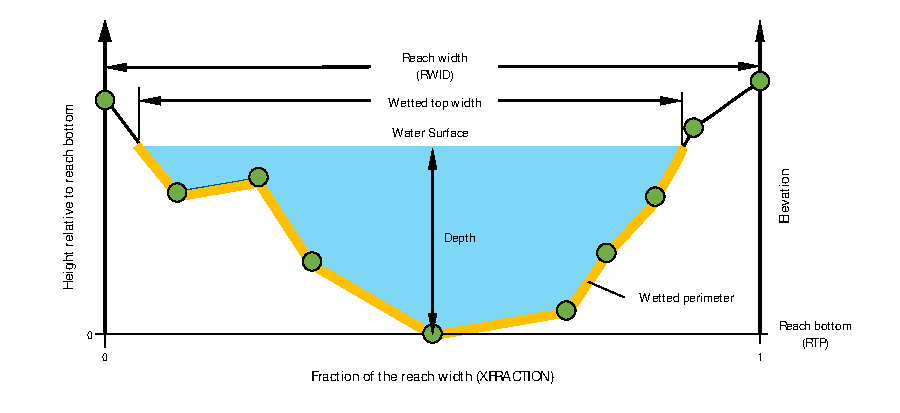
\includegraphics[scale=1.0]{../Figures/n-point-cross-section}
	\caption[Illustration of a irregular cross section used to compute depth, wetted top width, wetted perimeter, and wetted cross-sectional area for a stream reach]{Irregular cross section used to compute depth, wetted top width, wetted perimeter, and wetted cross-sectional area for a stream reach for the case where the maximum XFRACTION is one}
	\label{fig:sfr-n-point}
\end{figure}

Cross-Section tables are specified by including file names in the CROSSSECTIONS or PERIOD blocks of the SFR Package for specific reaches.  These file names correspond to a Streamflow Routing cross-section table input file.  The format of the Streamflow Routing cross-section table input file is described here.

\vspace{5mm}
\subsubsection{Structure of Blocks}
\vspace{5mm}

\lstinputlisting[style=blockdefinition]{./mf6ivar/tex/utl-sfrtab-dimensions.dat}
\lstinputlisting[style=blockdefinition]{./mf6ivar/tex/utl-sfrtab-table.dat}
\vspace{5mm}

\vspace{5mm}
\subsubsection{Explanation of Variables}
\begin{description}
% DO NOT MODIFY THIS FILE DIRECTLY.  IT IS CREATED BY mf6ivar.py 

\item \textbf{Block: DIMENSIONS}

\begin{description}
\item \texttt{nrow}---integer value specifying the number of rows in the reach cross-section table. There must be NROW rows of data in the TABLE block.

\item \texttt{ncol}---integer value specifying the number of columns in the reach cross-section table. There must be NCOL columns of data in the TABLE block. NCOL must be equal to 2 if MANFRACTION is not specified or 3 otherwise.

\end{description}
\item \textbf{Block: TABLE}

\begin{description}
\item \texttt{xfraction}---real value that defines the station (x) data for the cross-section as a fraction of the width (RWID) of the reach. XFRACTION must be greater than or equal to zero but can be greater than one. XFRACTION values can be used to decrease or increase the width of a reach from the specified reach width (RWID).

\item \texttt{height}---real value that is the height relative to the top of the lowest elevation of the streambed (RTP) and corresponding to the station data on the same line. HEIGHT must be greater than or equal to zero and at least one cross-section height must be equal to zero.

\item \texttt{manfraction}---real value that defines the Manning's roughness coefficient data for the cross-section as a fraction of the Manning's roughness coefficient for the reach (MAN) and corresponding to the station data on the same line. MANFRACTION must be greater than zero. MANFRACTION is applied from the XFRACTION value on the same line to the XFRACTION value on the next line. Although a MANFRACTION value is specified on the last line, any value greater than zero can be applied to MANFRACTION(NROW). MANFRACTION is only specified if NCOL is 3. If MANFRACTION is not specified, the Manning's roughness coefficient for the reach (MAN) is applied to the entire cross-section.

\end{description}


\end{description}

\subsubsection{Example Input File}
\lstinputlisting[style=inputfile]{./mf6ivar/examples/utl-sfrtab-example.dat}



\newpage
\subsection{Lake (LAK) Package}
\input{gwf/lak}

\newpage
\subsection{Unsaturated Zone Flow (UZF) Package}
\input{gwf/uzf}

\newpage
\subsection{Water Mover (MVR) Package}
The MVR Package can be used to transfer water from a provider to a receiver.  Providers are extraction wells, streamflow routing reaches, lakes and other model features that can be conceptualized as having water available.  The list of packages that can provide water to the MVR Package are:

\begin{itemize}
  \item Well Package
  \item Drain Package
  \item River Package
  \item General-Head Boundary Package
  \item Multi-Aquifer Well Package
  \item Streamflow Routing Package
  \item Unsaturated Zone Flow Package
  \item Lake Package
\end{itemize}

Receivers are package features within the model that solve a continuity equation of inflows, outflows, and change in storage.  These features include multi-aquifer wells, streamflow routing reaches, lakes, and unsaturated zone flow cells.  The list of packages that can receive water is shorter than the provider list, because the WEL, DRN, RIV, and GHB Packages do not represent a continuity equation (boundary stages or elevations are specified by the user).  Therefore, the list of packages that can act as receivers are:

\begin{itemize}
  \item Multi-Aquifer Well Package
  \item Streamflow Routing Package
  \item Unsaturated Zone Flow Package
  \item Lake Package
\end{itemize}

\noindent The program will terminate with an error if the MVR is used with an unsupported package type.

The MVR Package is based on the calculation of available water that can be moved from one package feature to another.  The equations used to determine how much water can be transferred are as follows, where $Q_P$ is the flow rate that can be supported by the provider (the available flow rate), and $Q_R$ is the actual rate of water transferred to the receiver.

\begin{enumerate}
\item A FACTOR can be specified such that 

$Q_R = \alpha Q_P$

\noindent where $\alpha$ is the factor to convert the provider flow rate to the receiver flow rate.

\item An EXCESS rate can be specified by the user as $Q_S$ such that

\[
    Q_R = 
\begin{cases}
    Q_P - Q_S, & \text{if } Q_P > Q_S \\
    0,              & \text{otherwise}
\end{cases}
\]

\noindent In the EXCESS case, any water that exceeds the user specified rate is provided to the receiver.  No water is provided to the receiver if the available water is less than the user specified value.

\item A THRESHOLD rate can be specified for $Q_S$ such that

\[
    Q_R = 
\begin{cases}
    0, & \text{if } Q_S > Q_P \\
    Q_S,              & \text{otherwise}
\end{cases}
\]

\noindent In the THRESHOLD case, no flow is provided to the receiver until the available water exceeds the user specified $Q_S$ rate.  Once the available water exceeds the user specified rate, then the $Q_S$ rate is provided to the receiver.

\item An UPTO rate can be specified for $Q_S$ such that

\[
    Q_R = 
\begin{cases}
    Q_S, & \text{if } Q_P > Q_S \\
    Q_P,              & \text{otherwise}
\end{cases}
\]

\noindent In the UPTO case, all of the available water will be taken from the provider up to the $Q_S$ value specified by the user.  Once $Q_S$ is exceeded, the receiver will continue to get the $Q_S$ value specified by the user.
\end{enumerate}

\noindent In the MVR PERIOD block (as shown below), the user assigns the equation used for each individual entry by specifying FACTOR, EXCESS, THRESHOLD, or UPTO to the input variable \texttt{mvrtype}.

Input to the Water Mover (MVR) Package is read from the file that has type ``MVR6'' in the Name File.  Only one MVR Package can be used per GWF Model.

\vspace{5mm}
\subsubsection{Structure of Blocks}
\vspace{5mm}

\noindent \textit{FOR EACH SIMULATION}
\lstinputlisting[style=blockdefinition]{./mf6ivar/tex/gwf-mvr-options.dat}
\lstinputlisting[style=blockdefinition]{./mf6ivar/tex/gwf-mvr-dimensions.dat}
\lstinputlisting[style=blockdefinition]{./mf6ivar/tex/gwf-mvr-packages.dat}
\vspace{5mm}
\noindent \textit{FOR ANY STRESS PERIOD}
\lstinputlisting[style=blockdefinition]{./mf6ivar/tex/gwf-mvr-period.dat}
All of the mover information in the PERIOD block will continue to apply for subsequent stress periods until the end of the simulation, or until another PERIOD block is encountered.  When a new PERIOD block is encountered, all of the movers from the previous block are replaced with the movers in the new PERIOD block.  Note that this behavior is different from the other advanced packages (MAW, SFR, LAK, and UZF).  To turn off all of the movers for a stress period, a PERIOD block must be specified with no entries.  If a PERIOD block is not specified for the first stress period, then no movers will be applied until the \texttt{iper} value of the first PERIOD block in the file.


\vspace{5mm}
\subsubsection{Explanation of Variables}
\begin{description}
\input{./mf6ivar/tex/gwf-mvr-desc.tex}
\end{description}

\vspace{5mm}
\subsubsection{Example Input File}
\lstinputlisting[style=inputfile]{./mf6ivar/examples/gwf-mvr-example.dat}


\newpage
\subsection{Ghost-Node Correction (GNC) Package}
\input{gwf/gnc}

\newpage
\subsection{Groundwater Flow (GWF) Exchange}
Input to the Groundwater Flow (GWF-GWF) Exchange is read from the file that has type ``GWF6-GWF6'' in the Simulation Name File.

The XT3D capability, which can be used to improve the accuracy of the flow calculation for certain types of cell connections and to represent anisotropic groundwater flow, is not implemented for the GWF-GWF Exchange.

\vspace{5mm}
\subsubsection{Structure of Blocks}
\lstinputlisting[style=blockdefinition]{./mf6ivar/tex/exg-gwfgwf-options.dat}
\lstinputlisting[style=blockdefinition]{./mf6ivar/tex/exg-gwfgwf-dimensions.dat}
\lstinputlisting[style=blockdefinition]{./mf6ivar/tex/exg-gwfgwf-exchangedata.dat}

\vspace{5mm}
\subsubsection{Explanation of Variables}
\begin{description}
\input{./mf6ivar/tex/exg-gwfgwf-desc.tex}
\end{description}

\vspace{5mm}
\subsubsection{Example Input File}
\lstinputlisting[style=inputfile]{./mf6ivar/examples/exg-gwfgwf-example.dat}

\vspace{5mm}
\subsubsection{Available observation types}
GWF-GWF Exchange observations include the simulated flow for any exchange (\texttt{flow-ja-face}). The data required for each GWF-GWF Exchange observation type is defined in table~\ref{table:gwf-gwfobstype}. For \texttt{flow-ja-face} observation types, negative and positive values represent a loss from and gain to the first model specified for this exchange.

\begin{longtable}{p{2cm} p{2.75cm} p{2cm} p{1.25cm} p{7cm}}
\caption{Available GWF-GWF Exchange observation types} \tabularnewline

\hline
\hline
\textbf{Exchange} & \textbf{Observation type} & \textbf{ID} & \textbf{ID2} & \textbf{Description} \\
\hline
\endhead

\hline
\endfoot

GWF-GWF & flow-ja-face & exchange number or boundname & -- & Flow between model 1 and model 2 for a specified exchange (which is the consecutive exchange number listed in the EXCHANGEDATA block), or the sum of these exchange flows by boundname if boundname is specified.
\label{table:gwf-gwfobstype}
\end{longtable}


\vspace{5mm}
\subsubsection{Example Observation Input File}
\lstinputlisting[style=inputfile]{./mf6ivar/examples/exg-gwfgwf-example-obs.dat}



